\documentclass{article}
\usepackage[utf8]{inputenc}
\usepackage{amsmath,amsthm,amssymb,amsfonts, fancyhdr, color, comment, graphicx, environ}
\usepackage{xcolor}
\usepackage[margin=2cm]{geometry}
\usepackage{listings}
\usepackage[many]{tcolorbox}
\usepackage{tikz} 
%-----------------------------------------------%
\newtcolorbox{codebox}[1][]{
  sharpish corners, % better drop shadow
  boxrule = 0pt,  % Remove all borders
  toprule = 1pt,   % Add a 1pt top rule (black by default)
  bottomrule = 1pt, % Add a 1pt bottom rule (black by default)
  enhanced,
  enlarge top by=0pt,  % No enlargement needed
  colback = yellow!10,   % Background color
  before skip = 0.2cm,  % Extra space before
  after skip = 0.5cm,   % Extra space after
  % Remove shadow and boxed title options
  #1,
}
%-----------------------------------------------%

%-----------------------------------------------%
\newcounter{pascalcode}[section]

\renewcommand{\thepascalcode}{\arabic{section}.\arabic{pascalcode}}

\lstdefinelanguage{pascal-like}{
  morekeywords={var, type, tuple, enumerate, fi, ret, downto, where, proc, fun, in, out, if, then, else, while, do, for, to, end, od},
  morecomment=[s]{\{-}{-\}},
  morestring=[b]",
  sensitive=true,
  keywordstyle=\color{orange},
  commentstyle=\color{green!70!black},
  stringstyle=\color{blue!70!black},
  backgroundcolor=\color{yellow!10},
  %numbers=left,
  %numberstyle=\tiny\color{gray},
  alsoletter={:,=,+,-,*,>,<,(,)},
  morekeywords=[2]{:,=,+,-,*,>,<,(,),&,&&,||,!,!=,==},
  keywordstyle=[2]{\color{blue}},
  literate={:=}{{\textcolor{green!50!black}{:=}}}2,
  morekeywords=[3]{nat, array, of, int, real, bool, char}, 
  keywordstyle=[3]{\color{blue!40!black}},
  mathescape=true
}

\lstnewenvironment{pascallike}[1][]{
  \refstepcounter{pascalcode}
  \lstset{
    language=pascal-like,
    %numbers=left,
    %numberstyle=\tiny\color{gray},
    %captionpos=b,
    #1
  }
}{}
%-----------------------------------------------%
\title{ \normalsize \textsc{Algoritmos y Estructuras\\
de Datos II}
		\\ [2.0cm]
		\HRule \\
		\LARGE \textbf{\uppercase{Ejercicios Resueltos - Práctico 1 - Ordenación Elemental}}
		\HRule \\ [0.5cm]
		\normalsize  \vspace*{5\baselineskip}}

\date{}

\author{Pedro Villar}
\begin{document}
%-----------------------------------------------%
\newcommand{\HRule}{\rule{\linewidth}{0.5pt}} % Define the \HRule command
\maketitle
%-----------------------------------------------%
\newpage
\section{Ejercicio 1}
Escribí algoritmos para resolver cada uno de los siguientes problemas sobre un arreglo a de posiciones $1$ a $n$, utilizando do. Elegí en cada caso entre estos dos encabezados el que sea más adecuado:

\begin{codebox}
\begin{pascallike}
proc nombre (in/out a: array [1..n] of nat)
    ...
end proc
\end{pascallike}
\end{codebox}
\begin{codebox}
\begin{pascallike}
proc nombre (out a: array [1..n] of nat)
    ...
end proc
\end{pascallike}
\end{codebox}
\begin{itemize}
    \item[(a)] Inicializar cada componente del arreglo con el valor $0$.
    \item[(b)] Inicializar el arreglo con los primeros $n$ números naturales positivos.
    \item[(c)] Inicializar el arreglo con los primeros $n$ números naturales impares.
    \item[(d)] Incrementar las posiciones impares del arreglo y dejar intactas las posiciones pares.  
\end{itemize}

\subsection{Solución (a)}
\begin{codebox}
\begin{pascallike}
proc inicializarConCero (out a: array [1..n] of nat)
    i := 1
    do i <= n -> 
    a[i] := 0
    i := i + 1
    od
end proc
\end{pascallike}
\end{codebox}

\subsection{Solución (b)}
\begin{codebox}
\begin{pascallike}
proc inicializarConNaturales (out a: array [1..n] of nat)
    i := 1
    do i <= n -> 
    a[i] := i
    i := i + 1
    od
end proc
\end{pascallike}
\end{codebox}

\subsection{Solución (c)}
\begin{codebox}
\begin{pascallike}
proc inicializarConImpares (out a: array [1..n] of nat)
    i := 1
    do i <= n -> 
    a[i] := 2 * i - 1
    i := i + 1
    od
end proc
\end{pascallike}
\end{codebox}

\subsection{Solución (d)}
\begin{codebox}
\begin{pascallike}
proc incrementarImpares (in/out a: array [1..n] of nat)
    i := 1
    do i <= n -> 
    if i mod 2 = 1 then
        a[i] := a[i] + 1
    fi
    i := i + 1
    od
end proc
\end{pascallike}
\end{codebox}

\section{Ejercicio 2}
Transformá cada uno de los algoritmos anteriores en uno equivalente que utilice \textbf{for...to} 

\subsection{Solución (a)}
\begin{codebox}
\begin{pascallike}
proc inicializarConCero (out a: array [1..n] of nat)
    for i := 1 to n do
    a[i] := 0
    od
end proc
\end{pascallike}
\end{codebox}

\subsection{Solución (b)}
\begin{codebox}
\begin{pascallike}
proc inicializarConNaturales (out a: array [1..n] of nat)
    for i := 1 to n do
    a[i] := i
    od
end proc
\end{pascallike}
\end{codebox}

\subsection{Solución (c)}
\begin{codebox}
\begin{pascallike}
proc inicializarConImpares (out a: array [1..n] of nat)
    for i := 1 to n do
    a[i] := 2 * i - 1
    od
end proc
\end{pascallike}
\end{codebox}

\subsection{Solución (d)}
\begin{codebox}
\begin{pascallike}
proc incrementarImpares (in/out a: array [1..n] of nat)
    for i := 1 to n do
    if i mod 2 = 1 then
        a[i] := a[i] + 1
    fi
    od
end proc
\end{pascallike}
\end{codebox}

\section{Ejercicio 3}
Escribí un algoritmo que reciba un arreglo a de posiciones 1 a n y determine si el arreglo recibido está ordenado o no. Explicá en palabras \textbf{qué} hace el algoritmo. Explicá en palabras \textbf{cómo} lo hace.

\subsection{Solución}
\begin{codebox}
\begin{pascallike}
fun estaOrdenado (a: array [1..n] of nat) ret r: bool
    r := true
    for i := 1 to n - 1 do
    if a[i] > a[i + 1] then
        r := false
    else
        skip
    fi
    od
end fun
\end{pascallike}
\end{codebox}

\textbf{¿Qué hace el algoritmo?} El algoritmo recibe un arreglo de números naturales y retorna un valor booleano que indica si el arreglo está ordenado o no.

\textbf{¿Cómo lo hace?} El algoritmo recorre el arreglo desde la primera posición hasta la penúltima, comparando cada elemento con el siguiente. Si encuentra un elemento mayor que el siguiente, retorna \textbf{false}, indicando que el arreglo no está ordenado. Si recorre todo el arreglo sin encontrar un elemento mayor que el siguiente, retorna \textbf{true}, indicando que el arreglo está ordenado.

\section{Ejercicio 4}

Ordená los siguientes arreglos, utilizando el algoritmo de ordenación por selección visto en clase. Mostrá en cada paso de iteración cuál es el elemento seleccionado y cómo queda el arreglo después de cada intercambio.

\begin{itemize}
    \item[(a)] $[7, 1, 10, 3, 4, 9, 5]$
    \item[(b)] $[5, 4, 3, 2, 1]$
    \item[(c)] $[1, 2, 3, 4, 5]$
\end{itemize}

\subsection{Solución (a)}
\begin{figure}[h]
    \centering
    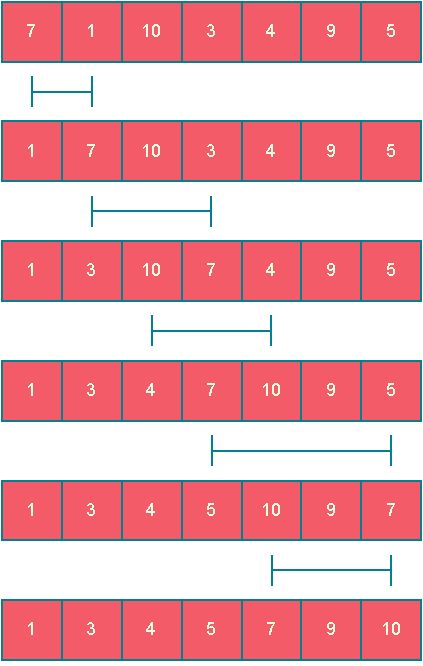
\includegraphics[scale=0.6]{estáticos/4a.pdf}
\end{figure}

\subsection{Solución (b)}
\begin{figure}[h]
    \centering
    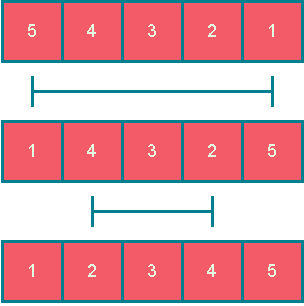
\includegraphics[scale=0.6]{estáticos/4b.pdf}
\end{figure}

\subsection{Solución (c)}
\begin{figure}[h]
    \centering
    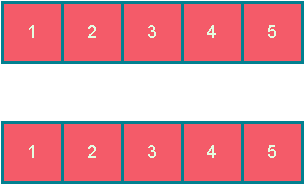
\includegraphics[scale=0.6]{estáticos/4c.pdf}
\end{figure}

\section{Ejercicio 5}
Calculá de la manera más exacta y simple posible el número de asignaciones a la variable t de los siguientes algoritmos. Las ecuaciones que se encuentran al final del práctico pueden ayudarte.
\begin{codebox}
\begin{pascallike}
t := 0
for i := 1 to n do
    for j := 1 to n^2 do
    for k := 1 to n^3 do
        t := t + 1
    od
    od
od
\end{pascallike}
\end{codebox}
\begin{codebox}
\begin{pascallike}
t := 0
for i := 1 to n do
    for j := 1 to i do
    for k := j to j+3 do
        t := t + 1
    od
    od
od
\end{pascallike}
\end{codebox}

\subsection{Solución (a)}

\begin{codebox}
\begin{pascallike}
ops(t := 0
for i := 1 to n do
    for j := 1 to n^2 do
    for k := 1 to n^3 do
        t := t + 1
    od
    od
od)
\end{pascallike}
\end{codebox}

Escribo el bucle en forma de sumatorias 
\begin{equation*}
  \sum_{i=1}^{n} \left(  \sum_{j=1}^{n^2} \left) \sum_{k=1}^{n^3} t := t+1 \right) \right)
\end{equation*}

Ahora aplico la función ops a la secuencia:

\begin{equation*}
  ops(t := 0) + \sum_{i=1}^{n} \left(  ops\left(\sum_{j=1}^{n^2} \sum_{k=1}^{n^3} t := t+1 \right) \right)
\end{equation*}

= \{ $ops=\sum_{j=1}^{n^2}$ es una sumatoria de $n^2$ elementos, por lo que vale $n^2$ \}

\begin{equation*}
  ops(t := 0) + \sum_{i=1}^{n} \left(  n^2 \cdot ops \left(\sum_{k=1}^{n^3} t := t+1 \right) \right)
\end{equation*}

= \{ $ops(t := 0)$ es una asignación, por lo que vale $1$ \}

\begin{equation*}
  1 + \sum_{i=1}^{n} \left(  n^2 \cdot ops \left(\sum_{k=1}^{n^3} t := t+1 \right) \right)
\end{equation*}

= \{ $ops \left(\sum_{k=1}^{n^3} t := t+1 \right)$ es una sumatoria de $n^3$ elementos, por lo que vale $n^3$ \}

\begin{equation*}
  1 + \sum_{i=1}^{n} \left(  n^2 \cdot n^3 \right)
\end{equation*}

= \{ Resuelvo la sumatoria interna \}

\begin{equation*}
  1 + \sum_{i=1}^{n} \left(  n^5 \right)
\end{equation*}

= \{ Resuelvo la sumatoria externa \}

\begin{equation*}
  1 + n \cdot n^5
\end{equation*}

= \{ Resuelvo la multiplicación \}

\begin{equation*}
  1 + n^6
\end{equation*}

\subsection{Solución (b)}

\begin{codebox}
\begin{pascallike}
ops(t := 0
for i := 1 to n do
    for j := 1 to i do
    for k := j to j+3 do
        t := t + 1
    od
    od
od)
\end{pascallike}
\end{codebox}

Escribo el bucle en forma de sumatorias
\begin{equation*}
  \sum_{i=1}^{n} \left(  \sum_{j=1}^{i} \left) \sum_{k=j}^{j+3} t := t+1 \right) \right)
\end{equation*}

Ahora aplico la función ops a la secuencia:

\begin{equation*}
  ops(t := 0) + \sum_{i=1}^{n} \left(  ops\left(\sum_{j=1}^{i} \sum_{k=j}^{j+3} t := t+1 \right) \right)
\end{equation*}

= \{ $ops=\sum_{j=1}^{i}$ es una sumatoria de $i$ elementos, por lo que vale $i$ \}

\begin{equation*}
  ops(t := 0) + \sum_{i=1}^{n} \left(  i \cdot ops \left(\sum_{k=j}^{j+3} t := t+1 \right) \right)
\end{equation*}

= \{ $ops(t := 0)$ es una asignación, por lo que vale $1$ \}

\begin{equation*}
  1 + \sum_{i=1}^{n} \left(  i \cdot ops \left(\sum_{k=j}^{j+3} t := t+1 \right) \right)
\end{equation*}

= \{ $ops \left(\sum_{k=j}^{j+3} t := t+1 \right)$ es una sumatoria de $4$ elementos, por lo que vale $4$ \}

\begin{equation*}
  1 + \sum_{i=1}^{n} \left(  4 \cdot i \right)
\end{equation*}

= \{ Resuelvo la sumatoria \}

\begin{equation*}
  1 + 4 \cdot \sum_{i=1}^{n} \left(  i \right)
\end{equation*}

= \{ Resuelvo la sumatoria \}

\begin{equation*}
  1 + 4 \cdot \frac{n \cdot (n+1)}{2}
\end{equation*}

= \{ Resuelvo la multiplicación \}

\begin{equation*}
  1 + 2 \cdot n \cdot (n+1)
\end{equation*}

= \{ Resuelvo la multiplicación \}

\begin{equation*}
  1 + 2 \cdot n^2 + 2 \cdot n
\end{equation*}

\section{Ejercicio 6}
Descifrá qué hacen los siguientes algoritmos, explicar cómo lo hacen y reescribirlos asignando nombres adecuados a todos los identificadores.

\begin{codebox}
\begin{pascallike}
proc p (in/out a: array [1..n] of T)
    var x: nat
    for i := n downto 2 do
    x := f(a,i)
    swap(a,i,x)
    od
end proc
\end{pascallike}
\end{codebox}

\begin{codebox}
\begin{pascallike}
fun f (a: array [1..n] of T, i: nat) ret x: nat
    x := 1
    for j := 2 to i do
    if a[j] > a[x] then
        x := j
    fi
    od
end fun
\end{pascallike}
\end{codebox}

\subsection{Solución (a)}
\textbf{Algoritmo p:} El algoritmo recibe un arreglo de elementos de tipo T y lo ordena de manera descendente. Para ello, recorre el arreglo desde la última posición hasta la segunda, en cada iteración busca el elemento más grande en el subarreglo que va desde la primera posición hasta la posición actual y lo intercambia con el elemento en la posición actual.
Se podria escribir de la siguiente manera:

\begin{codebox}
\begin{pascallike}
proc ordenarDescendente (in/out a: array [1..n] of T)
    var posMax: nat
    for i := n downto 2 do
    posMax := buscarMaximo(a,i)
    swap(a,i,posMax)
    od
end proc
\end{pascallike}
\end{codebox}

\subsection{Solución (b)}
\textbf{Función f:} La función recibe un arreglo de elementos de tipo T y un número natural $i$, y retorna la posición del elemento más grande en el subarreglo que va desde la primera posición hasta la posición $i$. Para ello, recorre el subarreglo desde la segunda posición hasta la posición $i$, en cada iteración compara el elemento actual con el elemento más grande encontrado hasta el momento y si el elemento actual es mayor, actualiza la posición del elemento más grande.
Se podria escribir de la siguiente manera:

\begin{codebox}{Solución (b)}
\begin{pascallike}
fun buscarMaximo (a: array [1..n] of T, i: nat) ret posMax: nat
    posMax := 1
    for j := 2 to i do
    if a[j] > a[posMax] then
        posMax := j
    fi
    od
end fun
\end{pascallike}
\end{codebox}

\section{Ejercicio 7}
Ordená los arreglos del ejercicio 4 utilizando el algoritmo de ordenación por inserción. Mostrá en cada paso de iteración las comparaciones e intercambios realizados hasta ubicar el elemento en su posición.

\subsection{Solución (a)}
\begin{figure}[h]
    \centering
    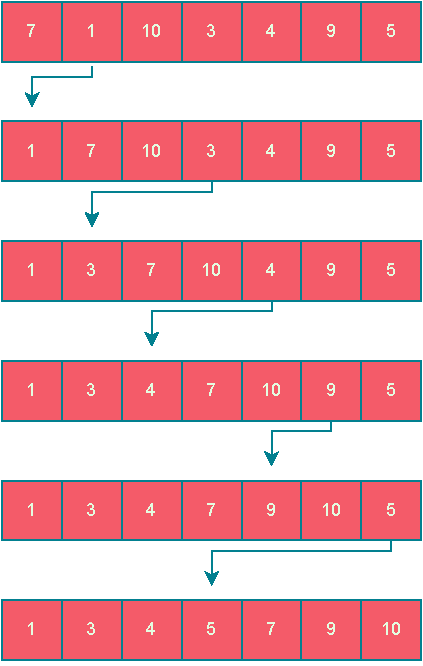
\includegraphics[scale=0.6]{./estáticos/7a.pdf}
\end{figure}

\subsection{Solución (b)}
\begin{figure}[h]
    \centering
    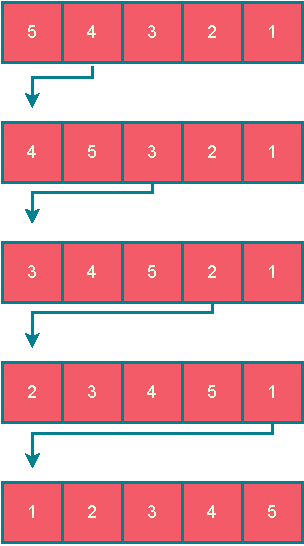
\includegraphics[scale=0.6]{./estáticos/7b.pdf}
\end{figure}

\subsection{Solución (c)}
\begin{figure}[h]
    \centering
    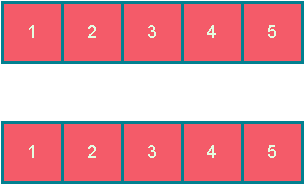
\includegraphics[scale=0.6]{./estáticos/7c.pdf}
\end{figure}

\section{Ejercicio 8}
Calculá el orden del número de asignaciones a la variable t de los siguientes algoritmos.

\begin{codebox}
\begin{pascallike}
t := 1
do t < n 
    t := t * 2
od
\end{pascallike}
\end{codebox}

\begin{codebox}
\begin{pascallike}
t := n
do t > 0 do
    t := t div 2
od
\end{pascallike}
\end{codebox}

\begin{codebox}
\begin{pascallike}
for i := 1 to n do
    t := i
    do t > 0 do
    t := t div 2
    od
od
\end{pascallike} 
\end{codebox}

\begin{codebox}
\begin{pascallike}
for i := 1 to n do
    t := i
    do t > 0 do
    t := t - 2
    od
od
\end{pascallike}
\end{codebox}

\subsection{Solución (a)}
El algoritmo realiza una asignación y luego realiza una multiplicación en cada iteración. El número de iteraciones es el menor número $k$ tal que $2^k \geq n$. Por lo tanto, el orden del número de asignaciones es $O(\log_2 n)$.

\subsection{Solución (b)}
El algoritmo realiza una asignación y luego realiza una división en cada iteración. El número de iteraciones es el menor número $k$ tal que $n \div 2^k = 0$. Por lo tanto, el orden del número de asignaciones es $O(\log_2 n)$.

\subsection{Solución (c)}
El algoritmo realiza una asignación y luego realiza una división en cada iteración. El número de iteraciones es el número $n$. Por lo tanto, el orden del número de asignaciones es $O(n \cdot \log_2 n)$.

\subsection{Solución (d)}
El algoritmo realiza una asignación y luego realiza una resta en cada iteración. El número de iteraciones es el número $n$. Por lo tanto, el orden del número de asignaciones es $O(n)$.


\section{Ejercicio 9}
Calculá el orden del número de comparaciones del algoritmo del ejercicio 3.

\subsection{Solución}

\begin{codebox}
\begin{pascallike}
fun estaOrdenado (a: array [1..n] of nat) ret r: bool
    for i := 1 to n - 1 do
    if a[i] > a[i + 1] then
        r := false
    else
        skip
    fi
    od
end fun
\end{pascallike}
\end{codebox}

El algoritmo realiza una comparación en cada iteración del bucle. El número de iteraciones es el menor número $k$ tal que $i + k \geq n-1$. Por lo tanto, el orden del número de comparaciones es $O(n)$.

$$ ops\left( \sum_{i=1}^{n-1} (if...else)) \right)$$
$$ ops\left( \sum_{i=1}^{n-1} 1 \right) = n$$

\section{Ejercicio 10}
Descifrá qué hacen los siguientes algoritmos, explicar cómo lo hacen y reescribirlos asignando nombres adecuados a todos los identificadores.

\begin{codebox}
\begin{pascallike}
proc q (in/out a: array [1..n] of T)
    for i := n-1 downto 1 do
    r(a,i)
    od
end proc
\end{pascallike}
\end{codebox}

\begin{codebox}
\begin{pascallike}
proc r (in/out a: array [1..n] of T, in i: nat)
    var j: nat
    j := i
    do j < n && a[j] > a[j+1] ->
    swap(a,j+1,j)
    j := j + 1
    od
end proc
\end{pascallike}
\end{codebox}

\subsection{Solución (a)}
\textbf{Algoritmo q:} El algoritmo recibe un arreglo de elementos de tipo T y lo ordena de manera ascendente. Para ello, recorre el arreglo desde la penúltima posición hasta la primera, en cada iteración llama a la función r con el arreglo y la posición actual.
Se podria escribir de la siguiente manera:

\begin{codebox}
\begin{pascallike}
proc ordenarAscendente (in/out a: array [1..n] of T)
    for i := n-1 downto 1 do
    ordenar(a,i)
    od
end proc
\end{pascallike}
\end{codebox}

\subsection{Solución (b)}
\textbf{Algoritmo r:} El algoritmo recibe un arreglo de elementos de tipo T y un número natural $i$, y realiza un intercambio entre el elemento en la posición $j$ y el elemento en la posición $j+1$ hasta que el elemento en la posición $j$ sea menor o igual que el elemento en la posición $j+1$ o hasta que la posición $j$ sea la última posición del arreglo.
Se podria escribir de la siguiente manera:

\begin{codebox}
\begin{pascallike}
proc ordenar (in/out a: array [1..n] of T, in i: nat)
    var j: nat
    j := i
    do j < n && a[j] > a[j+1] ->
    swap(a,j+1,j)
    j := j + 1
    od
end proc
\end{pascallike}
\end{codebox}

\end{document}